%*******10********20********30********40********50********60********70********80

% For all chapters, use the newdefined chap{} instead of chapter{}
% This will make the text at the top-left of the page be the same as the chapter

\chap{Generative Adversarial Network}
\section{Introduction}

The basic building block of this work is generative adversarial network. With the recent advancements in generative adversarial networks, it has become one the most studied generative model. A lot of variations and different architecture have been developed after the first paper was published.[cite][cite][cite]. In this chapter we explain GAN from the very basics. After reviewing this work, we discuss deep convolution generative adversarial network(DCGAN) which has pioneered the stabilization of the adversarial training.

\section{Generative Model}

Generative adversarial networks works on the principle of maximum likelihood.
%[https://arxiv.org/pdf/1701.00160.pdf].
It means when given a dataset, the model tries to provide probability distribution of the sample data parameterized by $\theta$. As this work is focused on computer vision,so the key relationship between images and statistics is that we can interpret images as samples from a high-dimensional probability distribution.
\par
It is very import to differentiate between explicit and implicit density model. So is tree differentiating  model based on maximum likelihood principal.
\begin{figure}[h]
    
    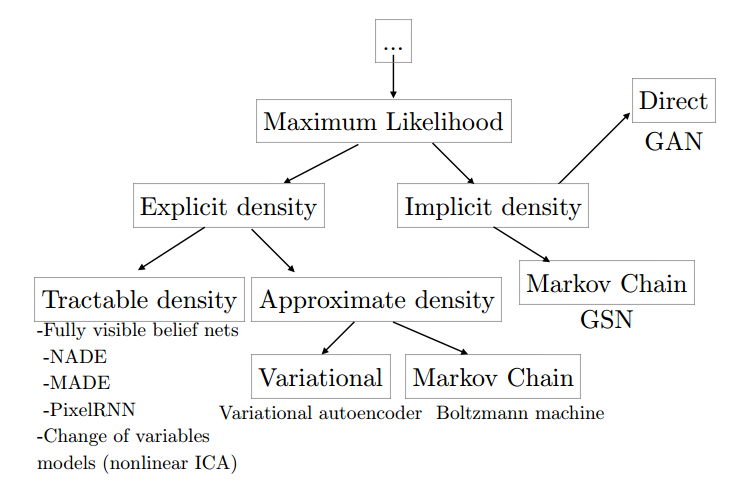
\includegraphics[scale=.6, angle=0]{Files/taxanomy.png}
    \caption[The panther]{Taxonomy of Generative Model\cite{GanTut}}
    \label{fig: jordan}
\end{figure}

In explicit model which also known as prescribed probabilistic model, we explicitly define the distribution of random variable and specify the log likelihood function.
In implicit model we don't need to define density function\cite{1}. The model learn the function from the data and generate sample in a single step.

\section{The GAN  Concept}
Generative Adversarial network works by inter playing two deep artificial neural networks, a generator(G) and a discriminator(D). Both of these network play a min max game, where generator tries to produce a fake image and discriminator tries to identify whether it is fake or real image as illustrated in Figure 3.1 
\begin{figure}[t]

  \centering
    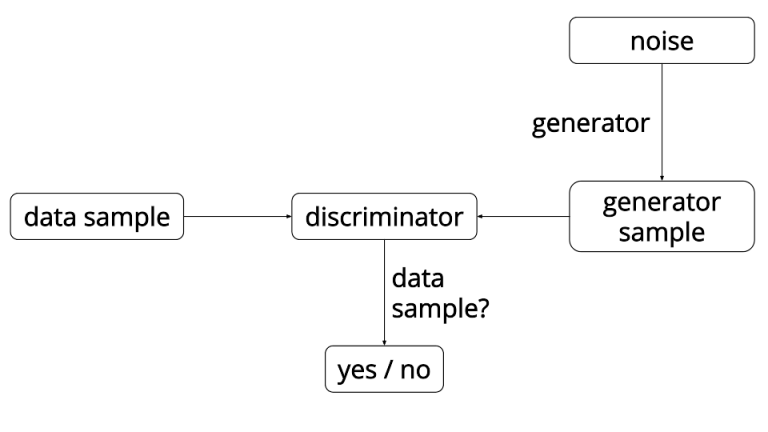
\includegraphics[scale=.4, angle=0]{Files/gan-overview.png}
    \caption[GAN overview]{ GAN overview\cite{Gan-overview}}
    \label{fig: GAN-Overview}
\end{figure}
\newpage
\subsection{Mathematical Definition}
Mathematically, let x,  $\theta_{G}$  and $\theta_{D}$ are be a data variable ,optimal hyper-parameters of the generator and discriminator model. Give a latent variable z drawn from a Gaussian distribution  , the genrator transform this variable to a sample from the data. And the discriminator tries to estimate whether the x is from data space $p_{data}$.
$$ F (\theta_{G}, \theta_{D}) = E_{x\sim p_{data}} [log (D (x; \theta_{D}))] + E_{z\sim N(0,I)}\log (1- D(G (z; \theta_{G}) ; \theta_{D}))$$
\subsection{Real World Example}
To understand GAN better,lets take a real world analogy. Suppose G is a counterfeit artist who produces fake money and D is a undercover agent from FBI who acting as buyer. The task of D is to differentiate the money. So to master the skill G, produces a fake currency batch and sells them to the D . If D identifies the batch then G updates its skill based on feedback fro the G. In this way  both goes back and forward, till G has learn the art of producing fake money.



